\mychapter{Estratégia de Varredura}
\label{Cap:Estrategia}

Quando se utiliza apenas uma aeronave para realizar a varredura de uma área de impacto em busca de possíveis embarcações não autorizadas, pode-se utilizar de diferentes estratégias de voo, por exemplo, o método de varredura em espiral ou o método de varredura vai e volta \cite{ost2012search}. 

Nesse primeiro método, a trajetória de voo é iniciada na extremidade da região e a aeronave percorrerá a área em espiral até o centro como mostra a figura \ref{fig:espiral}. 

\begin{figure} 
\center
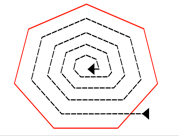
\includegraphics[width=0.5\textwidth]{espiral.png}
\caption{Método de Busca em Espiral.} 
\label{fig:espiral}
\end{figure} 

O segundo método realiza a varredura em linhas realizando curvas de 180 graus ao atingir a extremidade da área como mostra a figura \ref{fig:vaievolta}.

\begin{figure} 
\center
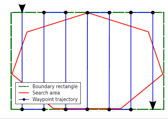
\includegraphics[width=0.5\textwidth]{vaievolta.png}
\caption{Método de Busca Vai e Volta.} 
\label{fig:vaievolta}
\end{figure} 

Em um cenário onde mais de um VANT será utilizado para a varredura de um área, há duas maneiras de acelerar a realização da missão, sendo elas realizar a inspeção com ou sem divisão em subárea. 

\section{Varredura sem Divisão em Subáreas}

Uma maneira de tomar proveito de uma rede multi VANTs para a varredura da área de impacto de foguetes seria realizar a missão na área por completo mantendo os VANTs voando a uma mesma velocidade e espaçados igualmente realizando o mesmo percurso, como mostra a figura \ref{fig:semsubdivisao}. Ambos velocidade e distância entre VANTs será relacionada ao ângulo de abertura da lenta da câmera utilizada, a velocidade do processamento de imagem, altura e velocidade de voo.

\begin{figure} 
\center
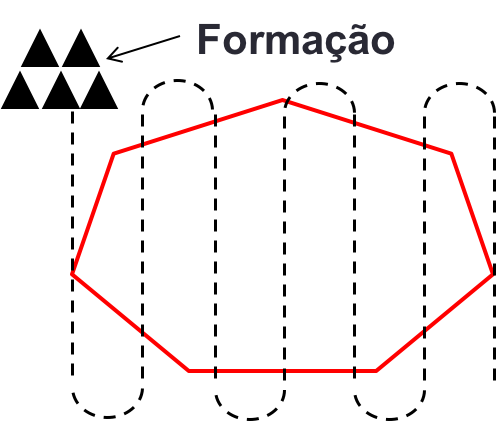
\includegraphics[width=0.5\textwidth]{semsubdivisao.png}
\caption{Varredura Vai e Volta sem Subdivisão de Área.} 
\label{fig:semsubdivisao}
\end{figure}

A utilização da estratégia sem divisão em subárea de varredura não há um considerável aumento de alcance da rede, pois os nós estarão sempre próximos. Por outro lado, em caso de perda de um nós o processo de reorganização é simples, bastando apenas aproximar os nós restantes. 

Uma decisão que pode ser tomada para aumentar o alcance da rede seria utilizar um nó de longo alcance e múltiplos nós de pequeno alcance, deixando a comunicação com a estação base a cargo do nó de maior alcance que funcionaria como \emph{hub} para os demais nós. Um ponto negativo dessa solução seria que caso o nó \emph{hub} perca conexão, os demais nós da rede também perderiam a conexão com a estação base. 

\section{Varredura com Divisão em Subáreas}

\begin{figure} 
\center
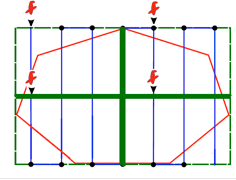
\includegraphics[width=0.5\textwidth]{comsubdivisao.png}
\caption{Varredura Vai e Volta com Subdivisão de Área.} 
\label{fig:comsubdivisao}
\end{figure}

Uma outra estratégia que poderia ser tomada seria dividir a área de varredura em subáreas de mesmo tamanho e utilizar os VANTs disponíveis para realizar a varredura de uma dessas subáreas como mostra a figura \ref{fig:comsubdivisao}. Nessa solução teríamos um aumento significante de alcance da rede, de modo que os pacotes serão transportados de nó em nó ate chegar a estação base ou nó de destino.

Em caso de perda de um dos nós da rede, a decisão a ser tomada para continuar a missão e garantir a varredura da área por completa não é tão trivial quando na estratégia de varredura sem divisão em subáreas, sendo necessário dividir novamente a área levando em consideração a área já varrida, como sugere \cite{marro2013path}.\\

Ambas as estratégias de varredura apresentadas nessa sessão possuem seus pontos negativos e positivos e a decisão de qual deles deve ser utilizada será função do operador do sistema de varredura. Na sessão a seguir serão discutidas as especificações técnicas do módulo Xbee adquirido pelo projeto.





